% !TeX spellcheck = pt_PT
%

\chapter{Aplicação Cliente} \label{cliente}

Este capítulo vai apresentar a nossa solução para o lado da aplicação cliente.

\section{Introdução e Estrutura da Aplicação Cliente} \label{sec41}
Como é observável na secção 2.3, a aplicação cliente é a segunda peça principal do nosso projeto. É onde se encontra a interface de utilizador, painéis de controlo e alguma lógica de negócio adicional.
No apêndice B é observável um diagrama em árvore da navegação da aplicação cliente.

Como descrito na secção 2.3, a aplicação cliente foi desenvolvida com o uso de \textit{Angular} e \textit{Ionic}. O tipo de organização e estrutura de uma aplicação cliente que o \emph{Angular} incentiva a aplicar é a estrutura \emph{Component} - \emph{Service}, e é esta estrutura que é seguida no nosso projeto.
As seguintes sub-secções explicam as ideias chaves de ambas as \textit{frameworks}.\\

\subsection{\textit{Angular Component} e \textit{NgModules}}\label{sub411}

Um \emph{Component} em \emph{Angular} é uma peça visual de uma aplicação, que pode estender deste uma página a uma tabela ou a um \textit{menu}. No caso da nossa aplicação cliente, cada especificação principal tem o seu componente. Dado que algumas regras de negócio implicam que certas páginas necessitem de componentes adicionais, como as estruturas \emph{Modal} ou \emph{Pop-over} que existem na \emph{Ionic Framework} (explicadas em detalhe na sub-secção 4.1.4), foi tomada como regra de decisão gerar estas estruturas num \emph{Component} separado do \emph{Component} principal das páginas, que são invocados nas circunstâncias apropriadas.

Cada \textit{Component} tem associado um \textit{template}, que representa o \textit{HTML} com a vista do componente, e um ficheiro \textit{TypeScript} que representa o objeto do próprio \textit{Component}, onde se encontram as definições das estruturas de dados internas do \textit{Component}, os \textit{imports} necessários ao \textit{Component}, assim como métodos chamados pelo \textit{template} com alguns comportamentos visuais, métodos que chamam os serviços que fazem o \textit{data-fetching}, métodos de \textit{redirect} da página, ou métodos que invocam os \textit{Controllers} dos componentes adicionais mencionados anteriormente.

Cada Component tem também o seu \textit{NgModule}. \textit{NgModules} são um tipo de estrutura disposta no \textit{Angular}, que ajuda a organizar a aplicação em módulos que podem ser importados ou importar outros módulos. A nossa aplicação cliente está assim estruturada para cada \textit{Component} ter o seu próprio módulo (os componentes adicionais são inseridos no mesmo módulo que o componente a que estão contextualmente associados), assim como o seu próprio \textit{routing module}, inserido dentro do módulo do componente, que trata do \textit{routing} dentro do módulo. Esta abordagem permite-nos ter o \textit{routing} todo da aplicação re-partido pelos módulos, em vez de estar todo centralizado num único componente.\\

\subsection{\textit{Angular Service}}\label{sub412}

Típicamente em arquitetura de \emph{software}, o termo \emph{Service} (ou serviço) é um termo utilizado para denominar uma peça de \emph{software} que tem um conjunto de funcionalidades específicas e limitadas, que estão por norma ligadas e contextualizadas, e que podem ser utilizadas e reutilizadas por diferentes partes de uma aplicação. 

No caso do \emph{Angular}, um \textit{Service} não é mais que uma classe onde são escritas funcionalidades, e que pode ser anotada como \emph{@Injectable} para que o \textit{Angular} consiga injectar essas funcionalidades num \textit{Component} através de um \textit{injector}. 

No caso da nossa aplicação cliente, cada entidade dispõe de um serviço \textit{HttpService} (agrupados no \textit{package} \textit{app/httpservices}) que contém todos os métodos que fazem as chamadas à \textit{web API} exposta pela aplicação servidora. 

Podemos observar no excerto de código seguinte, como exemplo, o serviço \textit{HttpEventService}.

\begin{lstlisting}
/* . . . */
export class EventService {
private BASE_URL = 'http://localhost:8080/event';
private httpOptions = {
headers: new HttpHeaders({
'Content-Type':  'application/json',
Authorization: 'my-auth-token',
'Access-Control-Allow-Origin': '*'
})
};

constructor(private http: HttpClient) { }

getEvents(): Observable<Event[]> {
const url = `${this.BASE_URL}/all`;
return this.http.get<Event[]>(url, this.httpOptions);
}

getEventsById(id: any) {
const url = `${this.BASE_URL}/findById/${id}`;
return this.http.get(url, this.httpOptions);
}
/* . . . */
\end{lstlisting}

Um dos aspetos principais dos serviços do \textit{Angular} são os \textit{Observables}. Os \textit{Observables} são um tipo de objetos implementados na biblioteca \textit{RxJS} que é utilizada pelo \textit{Angular}. Os \textit{Observables} atuam da mesma maneira que as \textit{Promises} (objeto \textit{Javascript} que representa a eventual conclusão de uma operação assíncrona e o seu resultado), com algumas diferenças chave: \\

\begin{tabular}{ll}
	\textit{Lazy} & Os \textit{Observables}, ao contrário das \textit{Promises}, são \textit{Lazy}. A função de\\
	& \textit{callback} passada ao \textit{Observable} só é invocada quando se chama o \\
	&método \textit{subscribe} do \textit{Observable}. \\
	\\
	\textit{Synchronous} & Os \textit{Observables} podem ser ambos síncronos e assíncronos, enquanto\\
	& que as \textit{Promises} são apenas assíncronas. \\
	\\
	Multiplos Valores & Os \textit{Observables} podem emitir multiplos valores. Um objeto \textit{Promise}\\
	& retorna sempre apenas um objeto (podendo este ser um \textit{array} de \\
	&valores, mas continua a ser um único objeto). Um \textit{Observable} pode \\
	&ser \textit{subscribed} a várias alturas da execução, e de cada vez que é \\
	&\textit{subscribed}, executa o seu comportamento novamente.\\
	\\
	\textit{Operators} & A biblioteca \textit{RxJS} apresenta um conjunto de \textit{operators} que podem \\
	&ser aplicados ao \textit{stream} do \textit{Observable} (como o \textit{map}). Este tipo de\\
	&comportamento não existe para \textit{Promises}.\\
	
	\\
\end{tabular}


Certas entidades dispõe tambem de um serviço próprio(agrupados no \textit{package} \textit{app/componentservices}) que contem todos os métodos que envolvem a algoritmia de regras de negócio adicionais dessas entidades. 
Podemos observar no troço de código seguinte, como exemplo, o serviço \textit{AthleteGameStatsService}, que contem um método \textit{getTotal()}, que retorna um objeto \textit{Stats} com o somatório de todos os \textit{Stats} dentro do array de \textit{AthleteGameStats}, utilizado na geração da tabela de estatísticas de um atleta. 

\begin{lstlisting}

import { Injectable } from '@angular/core';
import { AthleteGameStats } from "../../classes/associations/AthleteGameStats";
import { Stats } from "../../classes/stats";

@Injectable ({
providedIn: 'root'
})

export class AthleteGameStatsService {

constructor() { }

getTotal(stats: AthleteGameStats[]) {
let acc: Stats = new Stats();
Object.keys(acc).forEach( key => {
stats.forEach( stat => {
acc[key] += stat.stats[key];
});
});
return acc;}}
\end{lstlisting}

\subsection{\textit{Angular Data Binding}}\label{subsec413}

O \textit{Angular} também dispõe de um sistema de \textit{binding} de \textit{templates} que é utilizado com regularidade ao longo da aplicação. Dado que cada \textit{Component} tem a sua instância de classe e \textit{template} com a sua vista, o \textit{Angular} permite que estas vertentes comuniquem uma com a outra programáticamente através do chamado \textit{Data Binding}. 
Os principais tipos de \textit{Data Binding} que existem no \textit{Angular} são: \\

\begin{tabular}{ll}
	\emph{Interpolation} & Ligação de uma expressão a um elemento \textit{HTML} do \textit{template}. \\
	& A sintaxe deste \textit{binding} é {\{\{\textit{expression}\}\}}. \\
	\\
	\emph{Property} & Ligação de uma propriedade do \textit{Component} a um elemento \\
	&\textit{HTML} do \textit{template}. É uma ligação denominada \textit{Source-to-View}. \\
	& A sintaxe deste \textit{binding} é [\textit{target}]="\textit{expression}".\\
	\\
	\emph{Event} & Ligação de um evento de um elemento \textit{HTML} a uma declaração \\
	&do \textit{Component}. É uma ligação denominada \textit{View-to-Source}.\\
	& A sintaxe deste \textit{binding} é (\textit{target})="\textit{statement}".\\
	\\
	\emph{Two-Way} & Ligação dupla entre uma propriedade e um elemento. \\
	& O valor da propriedade transita até ao elemento, onde este pode ser \\
	&alterado através da interação do utilizador, e o novo valor transita de \\
	&volta até à propriedade. A sintaxe deste binding é [(\textit{target})]="\textit{expression}".\\
	\\
\end{tabular}
O \textit{Angular} também contém alguns tipos de \textit{binding} especializados para estilos. Estes tipos de \textit{binding} são utilizados quando se quer alterar programaticamente alguns aspetos visuais do \textit{template} sem querer fazer essa ligação a propriedades no \textit{Component}. Estes tipos especializados são:\\

\begin{tabular}{ll}
	\textit{Attribute} & Ligação de um atributo a um elemento \textit{HTML} do \textit{template}. A sintaxe deste\\
	& \textit{binding} é igual ao \textit{Property Binding}, substituindo o nome da propriedade\\
	& pelo nome do atributo [\textit{attr.atribute-name}]="\textit{expression}".\\
	\\
	\textit{Class} & Corresponde a ligar uma classe \textit{CSS} a um elemento \textit{HTML} do \textit{template}. \\
	&A sintaxe deste \textit{binding} é igual ao \textit{Property Binding}, substituindo \\
	&o nome da propriedade pelo nome da classe \textit{CSS} [\textit{class.name}]="\textit{expression}".\\
	\\
	\textit{Style} & Corresponde a ligar um estilo expecífico a um elemento \textit{HTML} do \textit{template}. \\
	&A sintaxe deste binding é igual ao Property Binding, substitundo o nome da \\
	&propriedade pelo nome do estilo [\textit{style.name}]="\textit{expression}";\\
\end{tabular}
\\
\\
\newpage

\subsection{\textit{IONIC API}}\label{subsec414}

A \textit{API} do \textit{Ionic} dispõe de uma lista de vários componentes visuais que podem ser intercalados com os do \textit{Angular} para criar uma aplicação responsiva e adaptável ao dispositivo em que é executada. Em [1] podemos encontrar a lista completa de todos os componentes disponíveis na \textit{API} do \textit{Ionic}. Ao longo deste projeto foram usados diversos componentes, nos casos que foram considerados apropriados, para garantir que eram cumpridas todas as regras de negócio aplicáveis, assim como garantir que a interface do utilizador seja clara e explícita na sua utilização.
Ao longo do desenvolvimento da aplicação cliente, foram utilizados diversos componentes em diversos contextos. No que toca a menus, foram utilizados:\\

\begin{tabular}{ll}
	\textit{ion-split-pane} & Menu lateral que aparece constantemente em toda a aplicação, onde \\
	&se encontram ligações para as diversas páginas.\\
	\\
	\textit{ion-tabs} & Barra de navegação, que aparece no \textit{footer} da página, com \textit{icons} com \\ &\textit{routing} para todas as páginas da aplicação. \\
	\\
	\textit{ion-header} & Barra de navegação, que aparece no \textit{header} da página, com uma \\
	&\textit{ion-toolbar} onde podem ser inseridos botões ou segmentos.\\
\end{tabular}

\begin{figure}[h]
	\begin{center}
		\resizebox{150mm}{!}{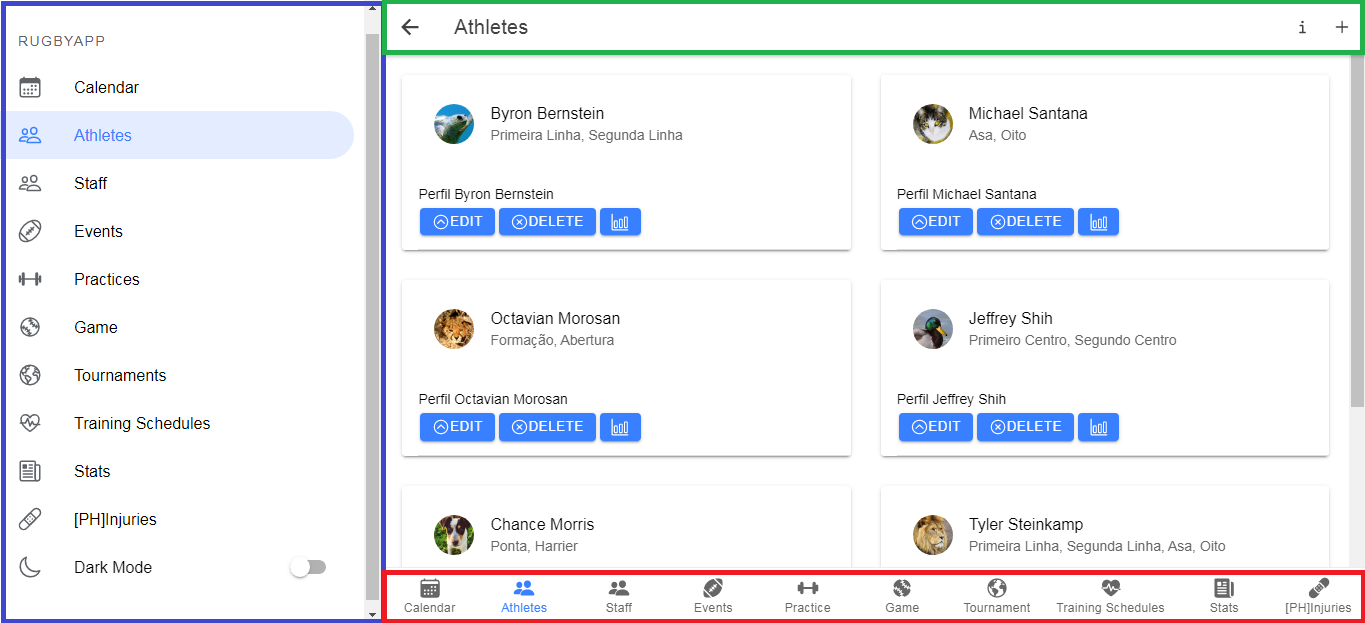
\includegraphics{./figures/frontend/MainComponent.png}}
	\end{center}
	\caption{Vista inicial da aplicação. Observa-se o \textit{ion-split-pane} a azul, o \textit{ion-tabs} a vermelho e o \textit{ion-header} a verde.}\label{fig:maincomponent}
\end{figure}

Como mencionado na secção 4.1.1, existem páginas na nossa aplicação cliente que requerem mais do que um \textit{Component} para garantir certas regras de negócios sem que a informação nas páginas fique sobrelotada e proporcionando a melhor experiência de utilização. Existem componentes na \textit{API} do \textit{Ionic} (alguns também mencionados na secção 4.1.1) que foram utilizados para este mesmo propósito:\\

\begin{tabular}{ll}
	\textit{ion-modal} & \textit{Dialog} (componente visual que se sobrepõe ao contexto atual da página e \\
	&requer interação do utilizador para desaparecer), normalmente utilizado \\
	&para apresentar uma página onde o utilizador tem diversas opções de interação.\\
	\\
	\textit{ion-popover} & \textit{Dialog} (assim como o \textit{ion-modal}) que é geralmente usado para conter acções \\
	&ou informação que não pode ser mostrada na totalidade sem comprometer\\
	& visualmente os elementos da página.\\
	\\
	\textit{ion-select} & Apesar de não requerer um \textit{controller} ou um \textit{component} próprio para ser \\
	&programado, o \textit{ion-select} é um \textit{ion-modal} pré-definido na \textit{API} exclusivamente \\
	&para \textit{input}/\textit{output} (ou seja, não é possível atribuir-lhe diretamente outro \\
	&comportamento que não o de dar ao utilizador diversas opções de escolha).\\
\end{tabular}

\begin{figure}[h]
	\begin{center}
		\resizebox{150mm}{!}{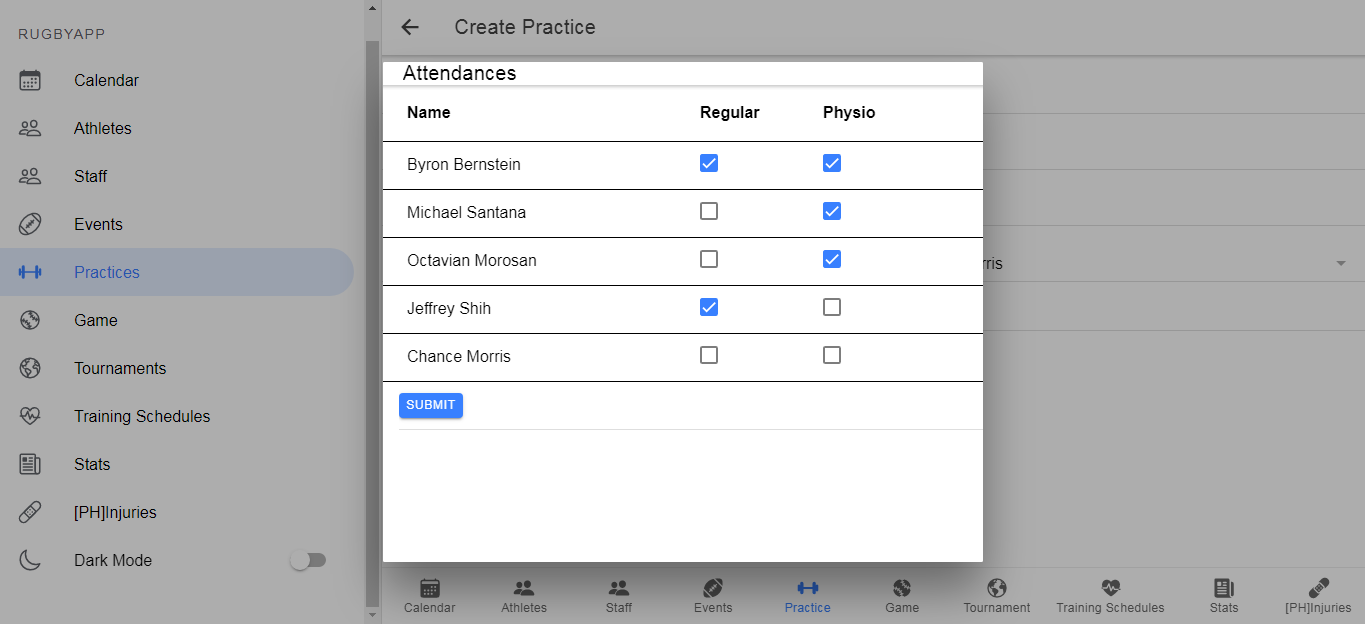
\includegraphics{./figures/frontend/PracticeFormPopover.png}}
	\end{center}
	\caption{\textit{Modal} da página do formulário de \textit{Practice}.}\label{fig:practiceformmodal}
\end{figure}
\newpage

\begin{figure}[h]
	\begin{center}
		\resizebox{150mm}{!}{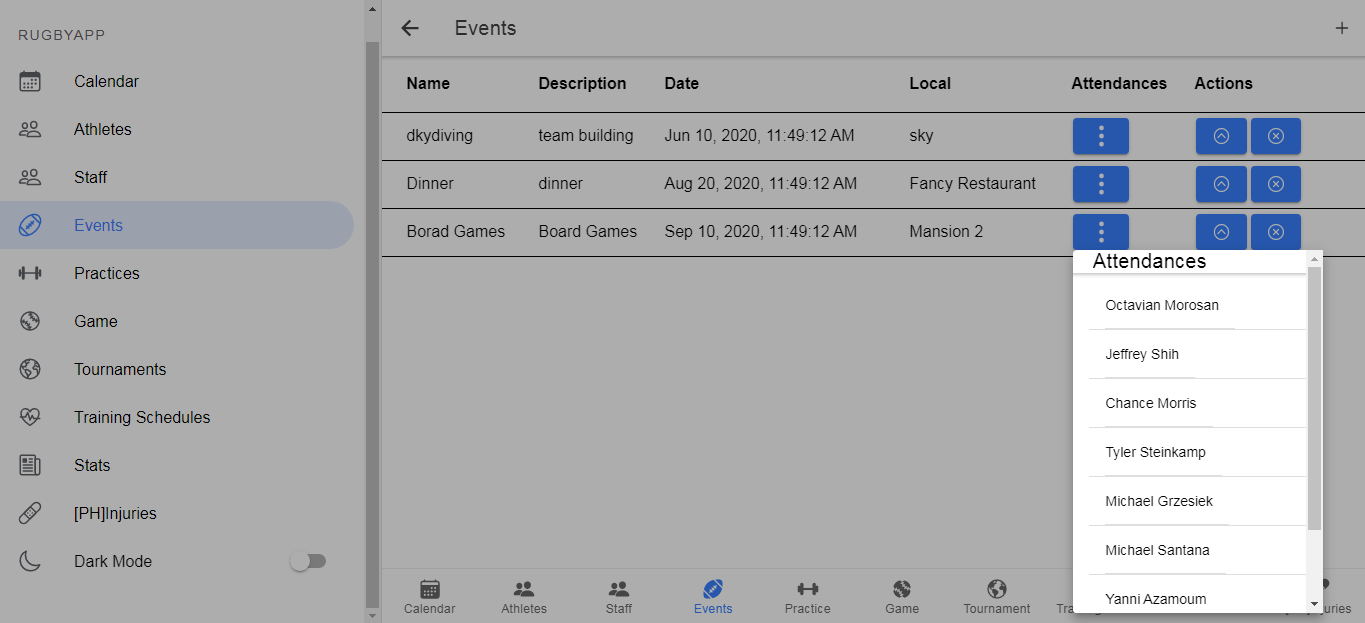
\includegraphics{./figures/frontend/EventPopover.png}}
	\end{center}
	\caption{\textit{Popover} da página \textit{Event}.}\label{fig:eventpopover}
\end{figure}

\begin{figure}[h]
	\begin{center}
		\resizebox{150mm}{!}{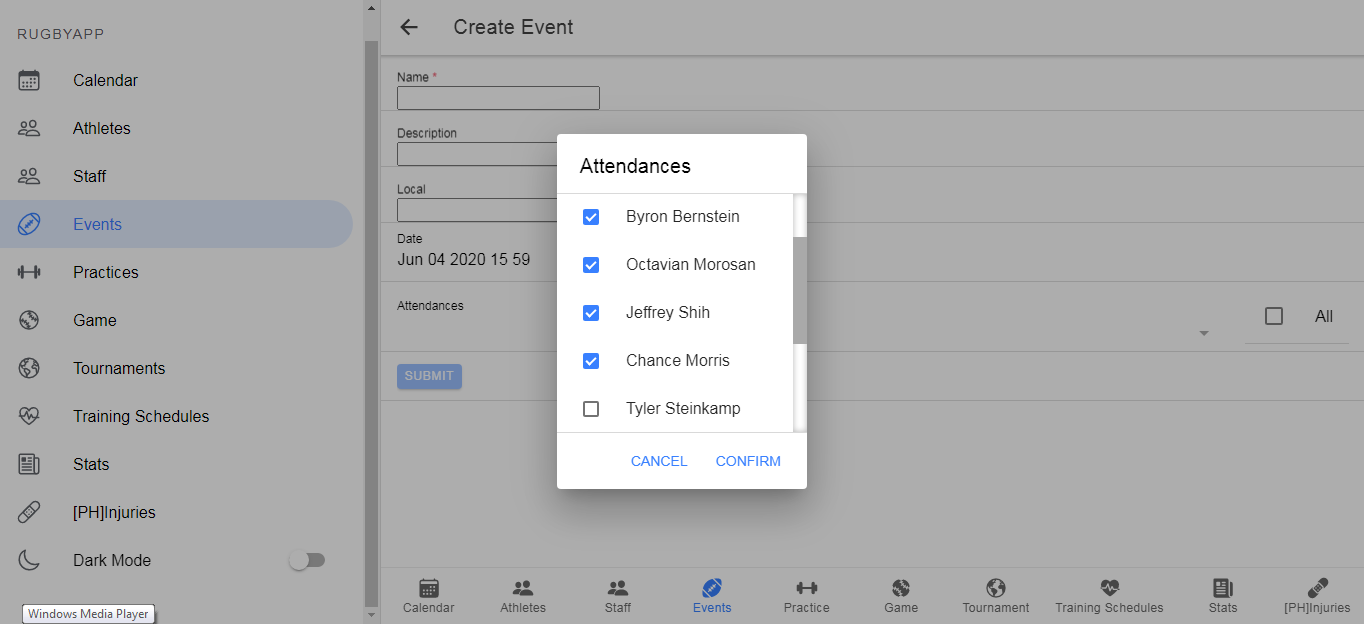
\includegraphics{./figures/frontend/EventFormSelect.png}}
	\end{center}
	\caption{\textit{Select} da página do formulário de \textit{Event}.}\label{fig:eventformselect}
\end{figure}
\newpage

Como referido anteriormente, ao contrário do \textit{ion-select}, o \textit{ion-modal} e o \textit{ion-popover} são componentes próprios e requerem um \textit{controller} para serem gerados e criados por outros componentes. Podemos observar no troço de código seguinte, o método \textit{createPopover()} inserido no \textit{event.component}

\begin{lstlisting}
constructor(private eventService: EventService, private popoverController: PopoverController, private alertController: AlertController) { }

/* . . .*/

async createPopover(profiles: Profile[], ev) {
const popover = await this.popoverController.create({
component: EventPopoverComponent,
componentProps: { profiles },
event: ev
});
return await popover.present();
}
\end{lstlisting}



O \textit{Component event.component} importa o módulo \textit{PopoverController} do \textit{package} do \textit{Ionic}, e cria a sua instância no construtor. Atribuindo o método \textit{createPopover} a um evento, é assim invocada a criação de um \textit{Popover}. 

\begin{lstlisting}
<ng-container matColumnDef="profiles">
<th mat-header-cell *matHeaderCellDef> Attendances </th>
<td mat-cell *matCellDef="let element">
<ion-button (click)="createPopover(element.profiles,$event)">
<ion-icon slot="icon-only" name="ellipsis-vertical"></ion-icon>
</ion-button>
</td>
</ng-container>
\end{lstlisting}



Cada elemento da coluna de \textit{Attendances} tem o seu próprio botão que vai criar o seu próprio \textit{Popover}. Passando a lista de \textit{Profiles} associadas a cada elemento, podemos criar um \textit{Popover} com cada uma das listas de \textit{Profiles} na tabela da página \textit{Event}.\\

\begin{lstlisting}
<ion-content>
<ion-list>
<ion-item *ngFor="let profile of this.navParams.get('profiles')">
/* . . . */
</ion-item>
</ion-list>
</ion-content>
\end{lstlisting}

Através de um módulo existente no package do \textit{Ionic}, chamado \textit{NavParams}, é possível passar informação ao \textit{Controller} do \textit{Popover}, e é possível do lado do \textit{Popover} obter essa informação para ser consumida. Neste caso, o Popover é meramente uma lista de itens com os nomes dos \textit{Profiles}, com um \textit{Link} para a página desse \textit{Profile}.

Do lado do \textit{ion-modal}, a ideia-chave é idêntica, exceto que o módulo que é importado pelo \textit{component} passa a ser o \textit{ModalController} em vez de \textit{PopoverController}. Continua-se a usar o \textit{NavParams} para passar informação ao \textit{Modal}.

\subsection{Angular Materials CDK}

O \textit{Angular} tambem dispõe de um \textit{CDK} (\textit{Component Dev Kit}) chamado \textit{Angular Materials}, onde encontramos vários componentes visuais. Em [2] podemos encontrar a lista completa de todos os componentes disponíveis neste \textit{CDK}. Apesar da nossa aplicação cliente explorar maioritariamente componentes da \textit{IONIC API}, também são usados alguns componentes deste \textit{CDK}, nomeadamente\\

\begin{tabular}{ll}
	\textit{mat-table} & Tabela usada para mostrar dados em diversas páginas da nossa \\
	&aplicação cliente, com a possibilidade de 
	adicionar comportamentos \\
	&adicionais à tabela, como paginação, linha de rodapé, filtro e ordenação. \\
	& \\
	\textit{mat-grid-list} & Grelha que permite variar os tamanhos que cada item ocupa na grelha,\\
	& ambos em número de colunas ou número de linhas, criando dinamismo \\
	&na organização da grelha sem a comprometer visualmente.\\
	& \\
	\textit{mat-form-field} & Componente que representa o campo de um formulário, onde se podem \\
	&aplicaram estilos de texto como \textit{Placeholder}, \textit{Hint} ou texto de erro. \\
	\\
\end{tabular}

Podemos observar no excerto de código seguinte o \textit{template} da \textit{mat-table} de \textit{Games}.

\begin{lstlisting}
<ion-content>
<table mat-table [dataSource]="this.dataSource" matSort class="mat-elevation-z8">

<ng-container matColumnDef="date">
<th mat-header-cell *matHeaderCellDef mat-sort-header> Date </th>
<td mat-cell *matCellDef="let element"> {{element.date | date:"medium"}} </td>
</ng-container>

/* . . . */

<tr mat-header-row *matHeaderRowDef="displayedColumns"></tr>
<tr mat-row *matRowDef="let row; columns: displayedColumns;"></tr>
</table>
</ion-content>
\end{lstlisting}
As \textit{mat-table} do \textit{Angular Materials} funcionam com base num objeto \textit{DataSource}. O \textit{Component} principal de cada página tem uma propriedade com este objeto, e após fazer \textit{data-fetching}, afeta esta propriedade com a informação para popular a tabela com os dados. Cada \textit{Component} tem também um \textit{array} com o nome das colunas da tabela. Da forma que o \textit{mat-table} é implementado, podemos organizar os nomes neste \textit{array} com a ordem que se pretende que as colunas sejam apresentados visualmente, e a tabela será desenhada com essa ordem, independentemente da ordem como está definido o HTML de cada coluna. \\


\begin{lstlisting}
export class GameComponent implements OnInit {
games: Game[];
displayedColumns: string[] = ['date', 'local', 'opponent', 'score', 'comment', 'athletes', 'actions'];
dataSource: any;
@ViewChild (MatSort, {static: true}) sort: MatSort;

/* . . . */

showGames() {
this.gameService.getGames().subscribe(games => {
this.games = games;
this.dataSource = new MatTableDataSource(this.games);
this.dataSource.sort = this.sort;
});
}
/* . . . */
}
\end{lstlisting}

\begin{figure}[h]
	\begin{center}
		\resizebox{150mm}{!}{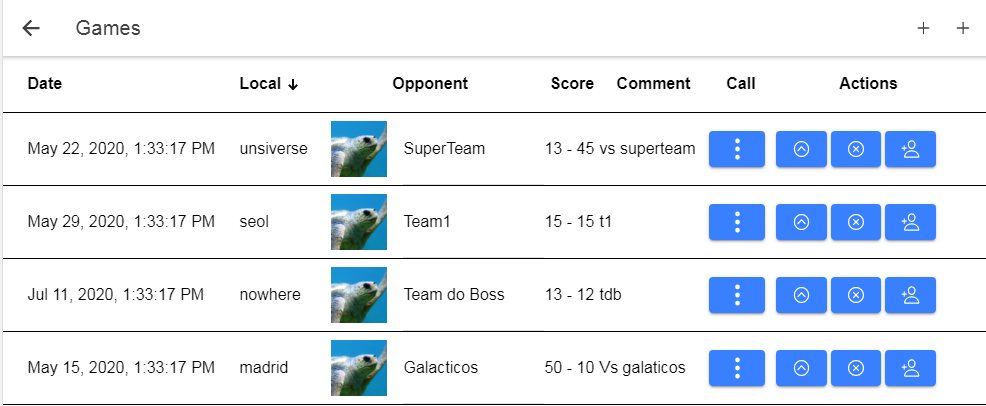
\includegraphics{./figures/frontend/GamesSortedNameDown.png}}
	\end{center}
	\caption{Tabela da página de \textit{Games}, ordenada decrescentemente por nome.}\label{fig:gamessortednameup}
\end{figure}



No que toca ao \textit{mat-grid-list}, podemos observar no troço de código seguinte como é que este componente é utilizado no \textit{Profile} de um \textit{Staff}.
\\

\begin{lstlisting}
<mat-grid-list cols="3" rowHeight="100px">
<mat-grid-tile [colspan]="1" [rowspan]="3">
<img [src]="staff?.profile.photo">
</mat-grid-tile>

<mat-grid-tile [colspan]="2" [rowspan]="1">
<ion-label>
<div class="ion-text-center"> <b> Nome </b> </div>
<div class="ion-text-center"> {{staff?.profile.name}} </div>
</ion-label>
</mat-grid-tile>

/* . . . */
</mat-grid-list>

\end{lstlisting}

Como referido anteriormente, uma das características chave do \textit{mat-grid-list} é a possibilidade de atribuir tamanhos diferentes aos diferentes items da grelha, permitindo-os organizar visualmente enquanto se mantem as proporções corretas da tabela. 

\begin{figure}[h]
	\begin{center}
		\resizebox{150mm}{!}{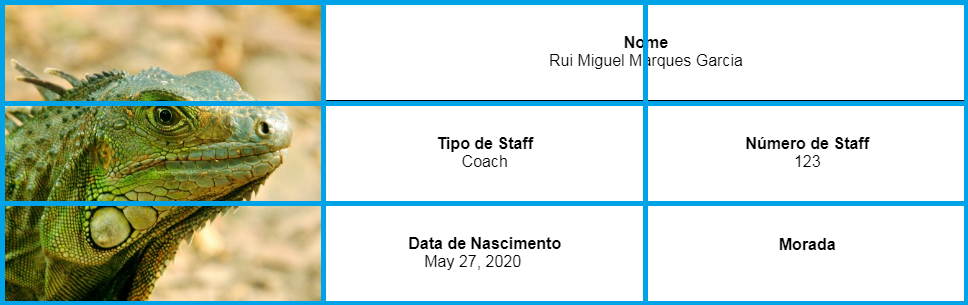
\includegraphics{./figures/frontend/StaffProfile.png}}
	\end{center}
	\caption{\textit{Profile} de um \textit{Staff}, com as linhas da grelha \textit{highlighted} para fins de visualização. }\label{fig:calendarall}
\end{figure}

É possível aferir, com base na imagem anterior, que a grelha gerada é uma grelha 3x3, no entanto, o item da imagem do perfíl ocupa 1x3, o nome do perfíl ocupa 2x1, e os restantes itens ocupam 1x1. É possível também aferir, apesar dos tamanhos variados, que a grelha fica organizada e ocupa espaço proporcional em ambos os eixos.\\

\subsection{Classes e Entidades}

Foram geradas na aplicação cliente as classes correspondentes às entidades da aplicação servidora em \emph{TypeScript}. Podemos observar no troço de código seguinte, como exemplo, a classe \emph{Event.ts} inserida no \emph{package} de classes da nossa Aplicação Cliente.

\begin{lstlisting}
export class Event {
constructor(
private id?: number,
private name?: string,
private description?: string,
private date?: Date,
private local?: string,
private profiles?: Profile[]
) {
this.id = id ? id : 0;
this.description = description ? description : '';
this.date = date ? date : new Date(0);
this.local = local ? local : '';
this.name = name ? name : '';
this.profiles = profiles ? profiles : [];
}
}
\end{lstlisting}

Um dos aspetos principais a salientar na implementação dos construtores das Entidades na aplicação cliente é a questão das propriedades poderem ser \emph{nullable}. Organizando os construtores para que todas as propriedades sejam \emph{nullable} enquanto se faz a verificação no corpo do construtor para a ausência destas propriedades, permite-se construir objetos atribuindo valores padrão a todas as propriedades que não existem na altura da criação. Este detalhe de implementação ajuda a gerar objetos vazios sem os problemas que ocorrem frequentemente na manipulação de valores \emph{null}.


\subsection{IONIC Lifecycle}

Em diversas partes da aplicação cliente, é necessário garantir que alguns comportamentos são executados em alturas específicas da geração e carregamento do componente da página. Por exemplo, em certas páginas que contém demasiada informação em relação ao tamanho da página, é necessário que o \textit{ion-split-pane} seja escondido para garantir que a página não fica visualmente comprometida pelo tamanho dos componentes que são mostrados. Para atingir este objetivo, o \textit{IONIC} dispõe de um \textit{lifecycle}, com vários ganchos que são executados em alturas específicas do carregamento do componente. Este \textit{lifecycle} segue a seguinte estrutura ordenada

\begin{tabular}{ll}
	\textit{constructor} & É executado quando a página é iniciada. É o melhor sitio \\
	&para definir valores \textit{default} para as variáveis do componente.\\
	\textit{ionViewDidLoad} & É executado quando a página foi carregada. Este evento é só \\
	&executado uma vez por cada criação de cada página. Se a página \\
	&for recarregada mas estiver em \textit{cache}, este evento não é executado\\
	& outra vez.\\
	\textit{ionViewWillEnter} & É executado quando a página está prestes a entrar e a tornar-se \\
	&a página ativa.\\
	\textit{ionViewDidEnter} & É executado quando a página entrou por completo e é agora a \\
	&página ativa. Este evento é sempre executado, independemente de \\
	&ser o primeiro carregamento da página ou se a página for \\
	&carregada da \textit{cache}.\\
	\textit{ionViewWillLeave} & É executado quando a página está prestes a sair e deixar de ser \\
	&a página ativa.\\
	\textit{ionViewDidLeave} & É executado quando a página acabou de sair e já não é a \\
	&página ativa.\\
	\textit{ionViewWillUnload} & É executado quando a página está prestes a ser destruída e os \\
	&seus elementos a serem removidos.\\
	\\
\end{tabular}

Seguindo o exemplo referido anteriormente, o \textit{ion-split-pane} é escondido no gancho \textit{ionViewDidEnter} e é recuperado no gancho \textit{ionViewDidLeave}.

\newpage

\subsection{\textit{Chart.js}}

A geração de gráficos é feita com base numa biblioteca chamada \textit{Chart.js}. \textit{Chart.js} é uma bibliteca \textit{open-source} com o foco príncipal em criar grafos responsivos. Em [3] encontramos a referência para esta biblioteca. 

Esta biblioteca contem a implementação de um objeto \textit{Chart}, que recebe, entre outra informação, o tipo de gráfico, as \textit{labels}, algumas opções de renderização, e \textit{Data Sets}. Cada \textit{Data Set} representa um bloco de informação no gráfico (no caso de um gráfico de barras, cada barra é um \textit{data set}, no caso de um gráfico de linhas, cada linha é um \textit{data set}).

\begin{figure}[h]
	\begin{center}
		\resizebox{130mm}{!}{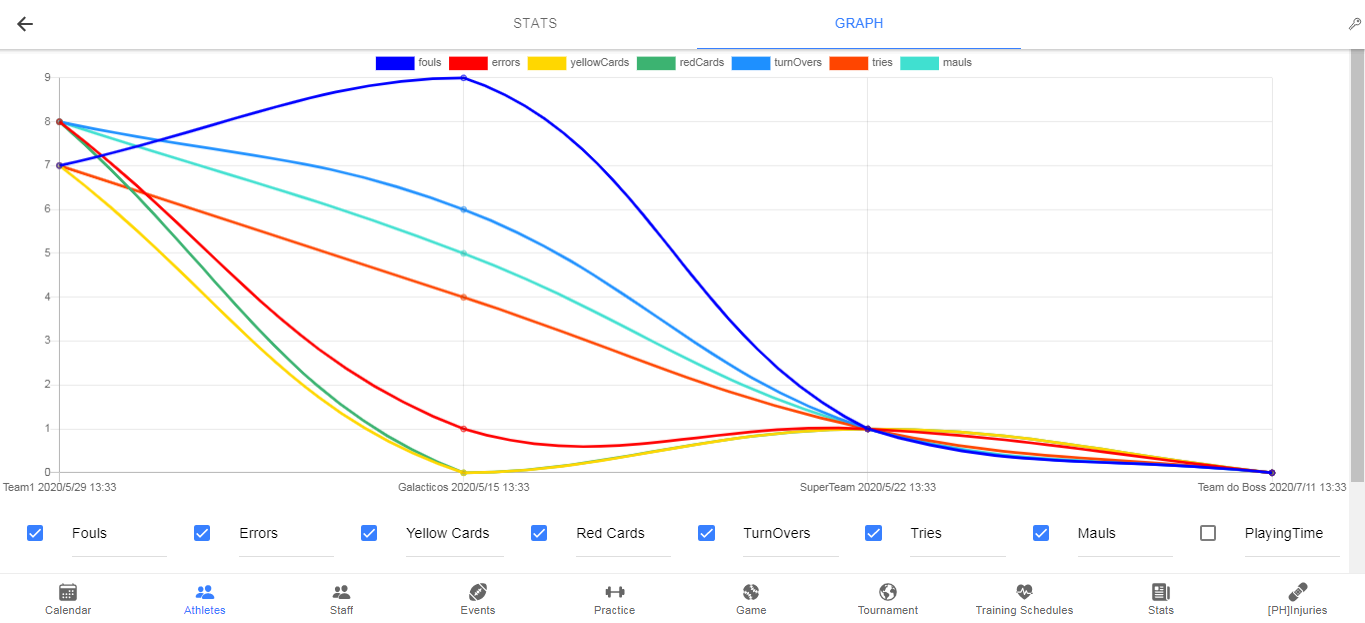
\includegraphics{./figures/frontend/graph.png}}
	\end{center}
	\caption{Aba \textit{Graph}, com as estatísticas \textit{Fouls}, \textit{Errors}, \textit{YellowCards}, \textit{RedCards}, \textit{turnOvers}, \textit{tries} e \textit{mauls} selecionados.}\label{fig:athleteprofile}
\end{figure}

\begin{figure}[h]
	\begin{center}
		\resizebox{130mm}{!}{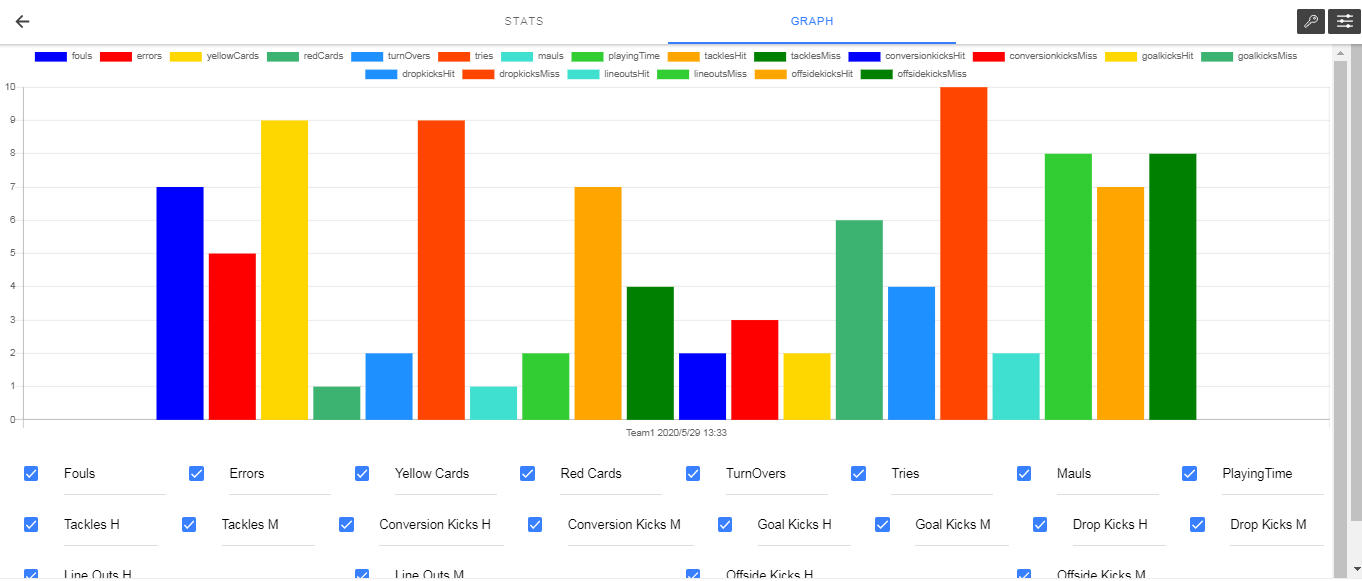
\includegraphics{./figures/frontend/graph2.png}}
	\end{center}
	\caption{Aba \textit{Graph}, com as estatísticas todas selecionadas. Quando o utilizador filtra os gráficos para apenas um atleta, a aplicação gera um gráfico de barras.}\label{fig:athleteprofile}
\end{figure}